\documentclass[aspectratio=169]{beamer}
\usetheme{Darmstadt}

\usepackage{amsmath, amssymb}
\usepackage{algorithm,algorithmicx,algpseudocode}
\usepackage{tikz}
\usetikzlibrary{matrix,decorations.pathmorphing,calc,decorations.pathreplacing,topaths,fit,positioning,automata,patterns,arrows,shapes,chains}
\tikzstyle{line} = [draw, -latex']

% Commands
\newcommand{\dd}{\,\text{d}}
\newcommand{\T}{\text{T}}
\newcommand{\B}[1]{\mathbf{#1}} % shortcut for \mathbf
\newcommand{\Bs}[1]{\boldsymbol{#1}} % shortcut for \boldsymbol
\newcommand{\pr}[1]{\left(#1\right)} % shortcut for \left(\right)
\newcommand{\br}[1]{\left[#1\right]} % shortcut for \left[\right]
\newcommand{\bbr}[1]{\left\{#1\right\}} % shortcut for \left\{\right\}
\newcommand{\nr}[1]{\left\|#1\right\|} % shortcut for \left\|\right\|

\title{High-Dimensional Gaussian Sampling}
\author{Yuejia Zhang}
\date{April 7, 2023}
\begin{document}
	
\begin{frame}
    \maketitle
\end{frame}

\section{Introduction} 
\subsection{Problem}
\begin{frame}
\frametitle{Problem Definition}
Sampling from a \(d\)-dimensional Gaussian distribution \(\mathcal{N}\pr{\Bs{\mu},\B{\Sigma}}\), where \(d\) may be large.

\[
    \pi(\Bs{\theta}) = \dfrac{1}{(2\pi)^{d/2}\text{det}(\B{\Sigma})^{1/2}}\exp\pr{-\dfrac{1}{2}(\Bs{\theta}-\Bs{\mu})^{\top}\B{\Sigma}^{-1}(\Bs{\theta}-\Bs{\mu})}.
\]

Covariance matrix \(\B{\Sigma}\) positive definite. Precision matrix \(\B{Q}=\B{\Sigma}^{-1}\) exists and also positive definite.
\end{frame}

\subsection{Motivation}
\begin{frame}
\frametitle{Special Cases}
\begin{itemize}
\item \(d = 1\)
\begin{algorithm}[H]
\caption{Box--Muller sampler}
\begin{algorithmic}[1]
\State Draw $u_1$, $u_2$ $\overset{\mathrm{i.i.d.}}{\sim} \mathcal{U}((0,1])$.
\State Set $\tilde{u}_1 = \sqrt{-2\log(u_1)}$.
\State Set $\tilde{u}_2 = 2\pi u_2$.\\ 
\Return $(\theta_1,\theta_2) = \pr{\mu + \frac{\tilde{u}_1}{\sqrt{q}} \sin(\tilde{u}_2),\mu + \frac{\tilde{u}_1}{\sqrt{q}} \cos(\tilde{u}_2)}$.
\end{algorithmic}
\end{algorithm}
\end{itemize}
\end{frame}

\begin{frame}
\frametitle{Special Cases}
\begin{algorithm}[H]
\caption{Sampler when $\B{Q}$ is a diagonal matrix}
\label{algo:multi_diag}
\begin{algorithmic}[1]
\For{$i \in [d]$} \Comment{\textcolor{blue}{In some programming languages, this loop can be vectorized.}} 
\State Draw $\displaystyle{\theta_i \sim \mathcal{N}\pr{\mu_i,1/q_i}}$.
\EndFor\\
\Return $\Bs{\theta} = (\theta_1,\cdots,\theta_d)^{\top}$.
\end{algorithmic}
\end{algorithm}
\end{frame}

\begin{frame}
\frametitle{General Cases}
\begin{algorithm}[H]
\caption{Cholesky sampler}
\begin{algorithmic}[1]
\State Set $\B{C} = \mathrm{chol}(\B{Q})$.
\Comment{\textcolor{blue}{$\B{Q} = \B{C}\B{C}^{\top}$}}
\State Draw $\B{z} \sim \mathcal{N}(\B{0}_d,\B{I}_d)$.
\State Solve $\B{C}^{\top}\B{w} = \B{z}$ w.r.t.\ $\B{w}$.\\
\Return $\Bs{\theta} = \Bs{\mu} + \B{w}$.
\end{algorithmic}
\end{algorithm}
Problem: 
\begin{itemize}
\item Storage requirement \(\Theta(d^2)\).
\item Computational cost \(\mathcal{O}(d^3 + d^2T)\) (\(T\) is the number of samples), only when \(\B{Q}\) is unchanged.
\end{itemize}
\end{frame}

\subsection{Methods}
\begin{frame}
\frametitle{More Efficient Solutions}
\begin{itemize}
    \item Square Root approximation: Approximate \(\B{Q}^{1/2}\).
    \item Conjugate Gradient: Solve a linear system w.r.t.\ \(\B{Q}\).
    \item Matrix Splitting: A generalization of Gibbs Sampler.
    \item Data Augmentation: Introduce auxiliary variable.
\end{itemize}
Improvement: computational cost $\mathcal{O}(d^2T)$ and storage requirement $\Theta(d)$.
\end{frame}

\subsection{Guidelines}
\begin{frame}
\frametitle{How to Choose the Sampler}

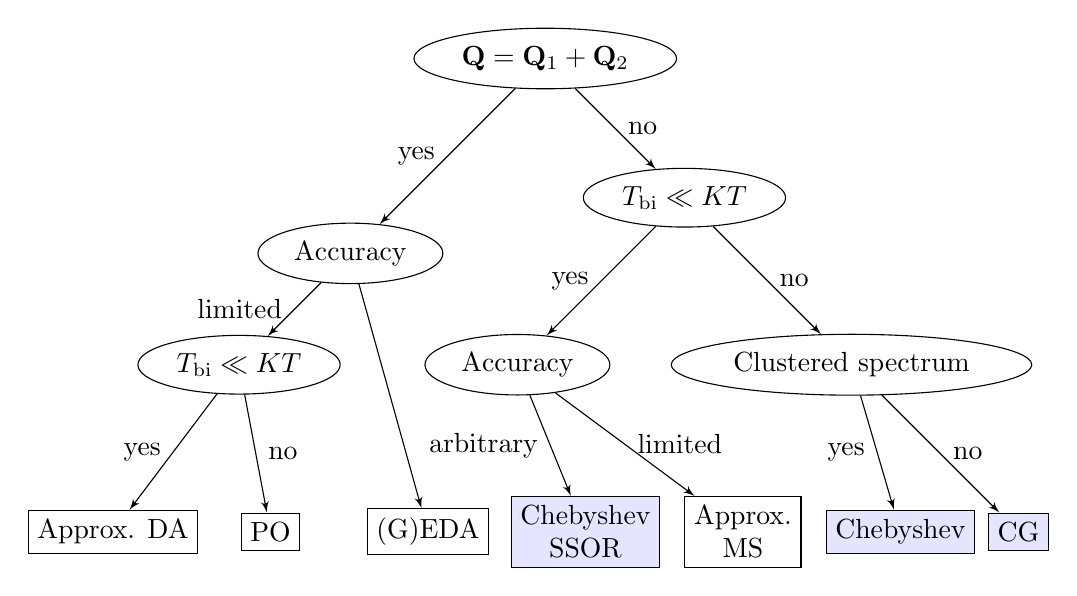
\begin{tikzpicture}[node distance=0.5cm, align=center]

\node (node0) [ellipse,draw=black] {$\B{Q} = \B{Q}_1 + \B{Q}_2$};

\node (node00) [ellipse,draw=black,below left of=node0, node distance=3.5cm] {Accuracy};
\path [line] (node0) -- node [midway,align=center,left=0.1em] {yes} (node00);

\node (node01) [ellipse,draw=black,below right of=node0, node distance=2.5cm] {$T_{\mathrm{bi}} \ll K T$};
\path [line] (node0) -- node [midway,align=center,right=0.1em] {no} (node01);

\node (node010) [ellipse,draw=black,below left of=node01, node distance=3cm] {Accuracy};
\path [line] (node01) -- node [midway,align=center,left=0.1em] {yes} (node010);

\node (node011) [ellipse,draw=black,below right of=node01, node distance=3cm] {Clustered spectrum};
\path [line] (node01) -- node [midway,align=center,right=0.1em] {no} (node011);

\node (node0111) [rectangle,fill=blue!10,draw=black,below right of=node011, node distance=3cm] {CG};
\path [line] (node011) -- node [midway,align=center,right=0.1em] {no} (node0111);

\node (node0110) [rectangle,fill=blue!10,draw=black,left of=node0111, node distance=1.5cm] {Chebyshev};
\path [line] (node011) -- node [midway,align=center,left=0.1em] {yes} (node0110);

\node (node0101) [rectangle,draw=black,left of=node0110, node distance=2cm] {Approx. \\ MS};
\path [line] (node010) -- node [midway,align=center,right=0.1em] {limited} (node0101);

\node (node0100) [rectangle,fill=blue!10,draw=black,left of=node0101, node distance=2cm] {Chebyshev \\ SSOR};
\path [line] (node010) -- node [midway,align=center,left=0.1em] {arbitrary} (node0100);

\node (node000) [rectangle,draw=black,left of=node0100, node distance=2cm] {(G)EDA};
\path [line] (node00) -- node [midway,align=center,right=0.1em] {} (node000);

\node (node001) [ellipse,draw=black,below left of=node00, node distance=2cm] {$T_{\mathrm{bi}} \ll K T$};
\path [line] (node00) -- node [midway,align=center,left=0.1em] {limited} (node001);

\node (node0011) [rectangle,draw=black,left of=node000, node distance=2cm] {PO};
\path [line] (node001) -- node [midway,align=center,right=0.1em] {no} (node0011);

\node (node0010) [rectangle,draw=black,left of=node0011, node distance=2cm] {Approx. DA};
\path [line] (node001) -- node [midway,align=center,left=0.1em] {yes} (node0010);


\end{tikzpicture}
\end{frame}

\section{Sampling Algorithms Derived From Numerical Algebra}
\subsection{Polynomial Approximation}
\begin{frame}
\frametitle{1}
\end{frame}
\subsection{Conjugate Gradient-Based Samplers}
\begin{frame}
\frametitle{1}
\end{frame}

\section{Sampling Algorithms Based On MCMC}
\subsection{Matrix Splitting}
\begin{frame}
\frametitle{1}
\end{frame}
\subsection{Data Augmentation}
\begin{frame}
\frametitle{1}
\end{frame}

\section{Unifying Approach Based On Stochastic PPA}
\subsection{PPA}
\begin{frame}
\frametitle{1}
\end{frame}

\end{document}